\documentclass{article}
\usepackage{graphicx}
\usepackage{wrapfig}
\usepackage{filecontents}
\usepackage{siunitx}
\usepackage[table]{xcolor}
\usepackage{float}
\usepackage{hyperref}
\usepackage{color} % balíček pro obarvování textů
\usepackage{xcolor}  % zapne možnost používání barev, mj. pro \definecolor
\hypersetup{
    colorlinks,
    linkcolor={red!50!black},
    citecolor={green!50!black},
    urlcolor={blue!80!black}
}
\definecolor{orange}{RGB}{ 251, 114, 032}
\definecolor{fialova}{RGB}{ 255, 000, 255} 

\usepackage{lmodern}
\usepackage{amssymb,amsmath}
\usepackage{ifxetex,ifluatex}
\usepackage{fixltx2e} % provides \textsubscript
\ifnum 0\ifxetex 1\fi\ifluatex 1\fi=0 % if pdftex
  \usepackage[T1]{fontenc}
  \usepackage[utf8]{inputenc}
\else % if luatex or xelatex
  \ifxetex
    \usepackage{mathspec}
  \else
    \usepackage{fontspec}
  \fi
  \defaultfontfeatures{Ligatures=TeX,Scale=MatchLowercase}
\fi



\usepackage[total={175mm,230mm}, top=23mm, left=20mm, includefoot]{geometry}
\usepackage{pgfplots} % http://www.chiark.greenend.org.uk/doc/texlive-doc/latex/pgfplots/pgfplots.pdf
\usepackage{blindtext}

\usepackage{subfiles} % Best loaded last in the preamble

\usepackage{bookmark}
\usepackage{tikz}
\usetikzlibrary{patterns}

\usepgfplotslibrary{polar}
\usepgfplotslibrary{external}
\usepgfplotslibrary{fillbetween}

\begin{document}
\begin{figure}[H]
    \vspace{-15mm}
    \centering
    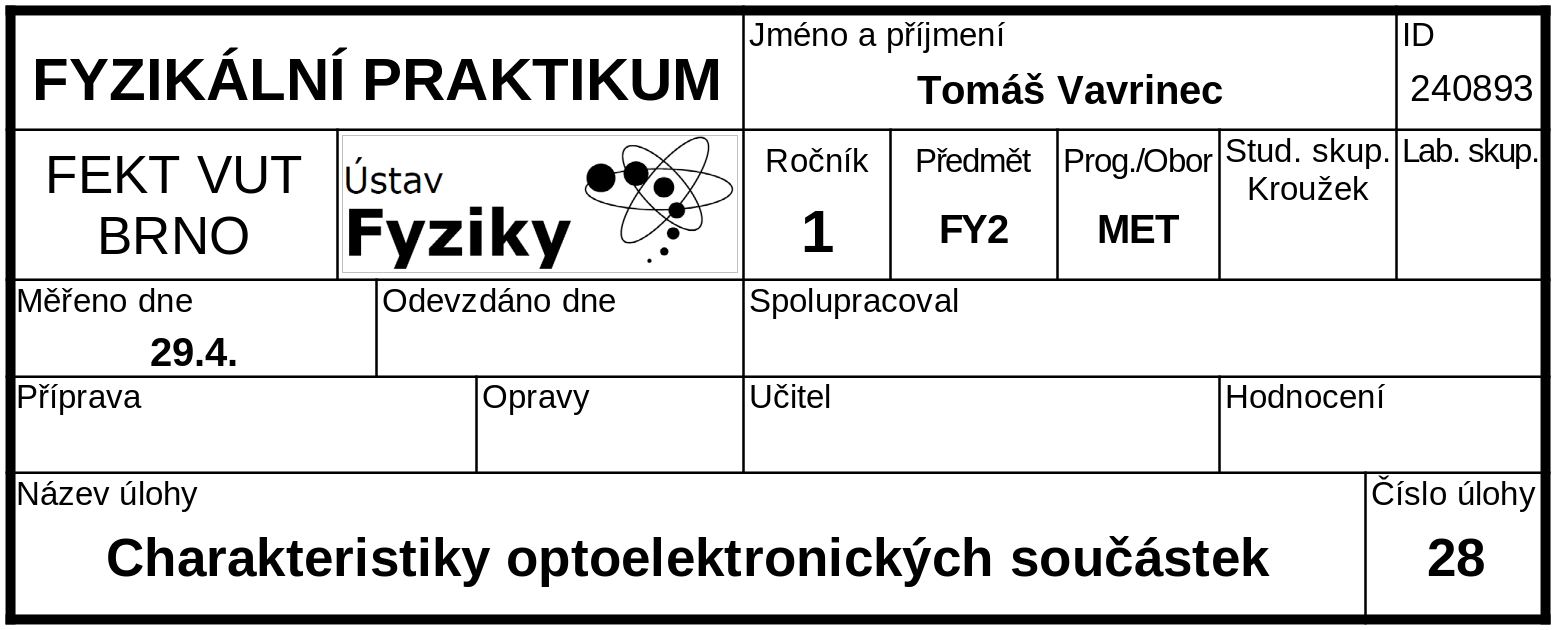
\includegraphics[width=\textwidth]{hlavička.png}
\end{figure}

\section{Úkol}
\begin{enumerate}
    \footnotesize
    \item Změřte voltampérovou, luxampérovou a\;směrovou vyzařovací charakteristiku luminiscenční diody, přenosovou charakteristiku optronu.
    Z grafu V-A charakteristiky určete součinitel \(n\)\;a\;\;přenosové charakteristiky určete kmitočtový rozsah optronu.

    \item Součástky o nichž pojednává tato úloha jsou polovodičové. 
    Připomeňte si základní znalosti o\;polovodičích ze střední školy, z\;předmětu Fyzika\;1\;a\;z\;úloh Teplotní závislost odporu polovodičového termistoru \;Hallův jev z Fyzikálního praktika 1.
\end{enumerate}

\section{Teoretický úvod}
\footnotesize
LED (Light Emitting Diode) je zdroj viditelného záření a záření v blízké infračervené oblasti.
Princip je založen na průchodu proudu skrz PN přechod, ve kterém rekombinují nosiče náboje.
Nosiče rekombinují ve chvíli, kdy je jejich energie menší než spodní hranice vodivostního pásu, neboli horní hranice zakázaného pásu.
Při rekombinaci se musí snížit potenciální energie elektronu o šířku zakázaného pásu, proto rekombinující elektron vyzáří foton o této energii.
Energie fotonu pak přímo odpovídá jeho vlnové délce podle vztahu.
\begin{equation}
    E_f=\frac{hc}{\lambda}\;\Rightarrow\;\lambda=\frac{hc}{E_f}
    \label{energie_fotonu}
\end{equation}
Kde \(h\) je Planckova konstanta, \(c\) je rychlost světla a \(\lambda\) je vlnové délka světla.
Vlnová délka světla, které vyzařuje LED, je proto určena šířkou zakázaného pásu.

Tento systém se dá použít i v opačném směru, mluvíme pak o fotodiodě namísto LED.
Foton, který dopadne do přechodu, vygeneruje vodivostní pár, který je okamžitě odsát elektrickým polem na přechodu.

\subsection{VA charakteristika}
VA charakteristika je přibližně popsatelná Schottkyho rovnicí 
\begin{equation}
    I_{led}=I_0\cdot(\exp{\frac{eU_{led}}{kTn}}-1)
    \label{schottkyho_rovnice}
\end{equation}
Kde \(I_0\) je saturační proud diody, \(e\) je elementární náboj, \(U_{led}\) je napětí na diodě, \(k\) Boltzmannova konstanta, \(T\) je teplota a \(n\) je číselný součinitel závislý na mechanizmu transportu.
Pro součinitel \(n\) platí \(1 < n < 2\).

\subsection{Luxampérová charakteristika}
Luxampérová charakteristika je závislost světelného toku tvořeného diodou \(\Phi\) na proudu diodou \(I_{led}\).
Světelný tok dopadá na fotodiodu, na které se tak přímoúměrně světelnému toku \(\Phi\) generuje napětí \(U_{det}\).
Závislost \(U_{det}\) na proudu \(I_{led}\) tak bude mít stejný tvar jako Luxampérová charakteristika a můžeme se tedy pro jednoduchost zaměnit.

\subsection{Směrová vyzařovací charakteristika}
Směrová vyzařovací charakteristika charakterizuje intenzitu světelného toku v závislosti na úhlu mezi snímačem a horizontální rovinou.

\subsection{Optron}
Optron je součástka složena z LED a fotodiody nebo fototranzistoru, která slouží např. pro galvanické oddělení. 

\section{Měření}
\subsection{Voltampérová a luxampérová charakteristika LED}
\begin{figure}[H]
	\begin{minipage}[t]{0.35\textwidth}
        
\begin{tabular}{|c|c|c|}
    \hline
    Iled~[A]	            & Uled~[V]	& Udet~[V]	 	            \\ \hline
    \(9.925\cdot10^{-7}\)	& \(1.339\)	& \(1.043\cdot10^{-5}\)	 	\\ \hline
    \(1.985\cdot10^{-6}\)	& \(1.375\)	& \(1.798\cdot10^{-5}\)	 	\\ \hline
    \(2.998\cdot10^{-6}\)	& \(1.395\)	& \(2.093\cdot10^{-5}\)	 	\\ \hline
    \(3.991\cdot10^{-6}\)	& \(1.410\)	& \(3.023\cdot10^{-5}\)	 	\\ \hline
    \(4.983\cdot10^{-6}\)	& \(1.421\)	& \(3.732\cdot10^{-5}\)	 	\\ \hline
    \(5.997\cdot10^{-6}\)	& \(1.431\)	& \(4.885\cdot10^{-5}\)	 	\\ \hline
    \(6.989\cdot10^{-6}\)	& \(1.438\)	& \(6.247\cdot10^{-5}\)	 	\\ \hline
    \(7.982\cdot10^{-6}\)	& \(1.445\)	& \(7.976\cdot10^{-5}\)	 	\\ \hline
    \(8.995\cdot10^{-6}\)	& \(1.451\)	& \(9.730\cdot10^{-5}\)	 	\\ \hline
    \(9.988\cdot10^{-6}\)	& \(1.456\)	& \(1.171\cdot10^{-4}\)	 	\\ \hline
    \(1.499\cdot10^{-5}\)	& \(1.476\)	& \(2.420\cdot10^{-4}\)	 	\\ \hline
    \(2.000\cdot10^{-5}\)	& \(1.491\)	& \(4.101\cdot10^{-4}\)	 	\\ \hline
    \(2.998\cdot10^{-5}\)	& \(1.510\)	& \(8.531\cdot10^{-4}\)	 	\\ \hline
    \(3.999\cdot10^{-5}\)	& \(1.523\)	& \(1.415\cdot10^{-3}\)	 	\\ \hline
    \(4.998\cdot10^{-5}\)	& \(1.533\)	& \(2.068\cdot10^{-3}\)	 	\\ \hline
    \(5.999\cdot10^{-5}\)	& \(1.541\)	& \(2.810\cdot10^{-3}\)	 	\\ \hline
    \(7.000\cdot10^{-5}\)	& \(1.548\)	& \(3.607\cdot10^{-3}\)	 	\\ \hline
    \(7.999\cdot10^{-5}\)	& \(1.553\)	& \(4.465\cdot10^{-3}\)	 	\\ \hline
    \(8.963\cdot10^{-5}\)	& \(1.562\)	& \(6.038\cdot10^{-3}\)	 	\\ \hline
    \(9.964\cdot10^{-5}\)	& \(1.566\)	& \(7.034\cdot10^{-3}\)	 	\\ \hline
    \(1.497\cdot10^{-4}\)	& \(1.581\)	& \(1.247\cdot10^{-2}\)	 	\\ \hline
    \(1.997\cdot10^{-4}\)	& \(1.592\)	& \(1.827\cdot10^{-2}\)	 	\\ \hline
    \(2.998\cdot10^{-4}\)	& \(1.607\)	& \(2.995\cdot10^{-2}\)	 	\\ \hline
    \(3.999\cdot10^{-4}\)	& \(1.617\)	& \(4.128\cdot10^{-2}\)	 	\\ \hline
    \(4.996\cdot10^{-4}\)	& \(1.625\)	& \(5.180\cdot10^{-2}\)	 	\\ \hline
    \(5.997\cdot10^{-4}\)	& \(1.631\)	& \(6.167\cdot10^{-2}\)	 	\\ \hline
    \(6.998\cdot10^{-4}\)	& \(1.636\)	& \(7.074\cdot10^{-2}\)	 	\\ \hline
    \(7.999\cdot10^{-4}\)	& \(1.641\)	& \(7.913\cdot10^{-2}\)	 	\\ \hline
    \(9.000\cdot10^{-4}\)	& \(1.645\)	& \(8.687\cdot10^{-2}\)	 	\\ \hline
    \(9.996\cdot10^{-4}\)	& \(1.649\)	& \(9.413\cdot10^{-2}\)	 	\\ \hline
    \(1.500\cdot10^{-3}\)	& \(1.653\)	& \(1.203\cdot10^{-1}\)	 	\\ \hline
    \(1.999\cdot10^{-3}\)	& \(1.676\)	& \(1.476\cdot10^{-1}\)	 	\\ \hline
    \(2.998\cdot10^{-3}\)	& \(1.693\)	& \(1.799\cdot10^{-1}\)	 	\\ \hline
    \(3.998\cdot10^{-3}\)	& \(1.706\)	& \(2.031\cdot10^{-1}\)	 	\\ \hline
    \(4.997\cdot10^{-3}\)	& \(1.717\)	& \(2.217\cdot10^{-1}\)	 	\\ \hline
    \(5.997\cdot10^{-3}\)	& \(1.727\)	& \(2.367\cdot10^{-1}\)	 	\\ \hline
    \(6.996\cdot10^{-3}\)	& \(1.737\)	& \(2.498\cdot10^{-1}\)	 	\\ \hline
    \(7.996\cdot10^{-3}\)	& \(1.745\)	& \(2.609\cdot10^{-1}\)	 	\\ \hline
    \(8.995\cdot10^{-3}\)	& \(1.753\)	& \(2.709\cdot10^{-1}\)	 	\\ \hline
    \(9.995\cdot10^{-3}\)	& \(1.760\)	& \(2.794\cdot10^{-1}\)	 	\\ \hline
    \(2.000\cdot10^{-2}\)	& \(1.832\)	& \(3.405\cdot10^{-1}\)	 	\\ \hline
\end{tabular}
    \end{minipage}
    \hfill
	\begin{minipage}[t]{0.63\textwidth}
        \pgfplotsset{width=105mm,compat=1.9}
        % \vspace*{-120mm}
        % \begin{tikzpicture}
%     \begin{axis}[
%         axis y line*=left,
%         title={Klasická AV charakteristika},
%         xlabel={\(U_{led}~[V]\)},
%         ylabel={\(I_{led}~[mA]\)},
%         xmin=1.3, xmax=1.85,
%         ymin=0, ymax=23,
%         legend pos=north west,
%     ]
%     \addplot[
%         only marks,
%         color=red,
%         mark=*,
%         ]
%         coordinates {
%             (1.339 ,9.925*10^-4)
%             (1.375 ,1.985*10^-3)
%             (1.395 ,2.998*10^-3)
%             (1.410 ,3.991*10^-3)
%             (1.421 ,4.983*10^-3)
%             (1.431 ,5.997*10^-3)
%             (1.438 ,6.989*10^-3)
%             (1.445 ,7.982*10^-3)
%             (1.451 ,8.995*10^-3)
%             (1.456 ,9.988*10^-3)
%             (1.476 ,1.499*10^-2)
%             (1.491 ,2.000*10^-2)
%             (1.510 ,2.998*10^-2)
%             (1.523 ,3.999*10^-2)
%             (1.533 ,4.998*10^-2)
%             (1.541 ,5.999*10^-2)
%             (1.548 ,7.000*10^-2)
%             (1.553 ,7.999*10^-2)
%             (1.562 ,8.963*10^-2)
%             (1.566 ,9.964*10^-2)
%             (1.581 ,1.497*10^-1)
%             (1.592 ,1.997*10^-1)
%             (1.607 ,2.998*10^-1)
%             (1.617 ,3.999*10^-1)
%             (1.625 ,4.996*10^-1)
%             (1.631 ,5.997*10^-1)
%             (1.636 ,6.998*10^-1)
%             (1.641 ,7.999*10^-1)
%             (1.645 ,9.000*10^-1)
%             (1.649 ,9.996*10^-1)
%             (1.653 ,1.500*10^0)
%             (1.676 ,1.999*10^0)
%             (1.693 ,2.998*10^0)
%             (1.706 ,3.998*10^0)
%             (1.717 ,4.997*10^0)
%             (1.727 ,5.997*10^0)
%             (1.737 ,6.996*10^0)
%             (1.745 ,7.996*10^0)
%             (1.753 ,8.995*10^0)
%             (1.760 ,9.995*10^0)
%             (1.832 ,20.000)
%             };
%     \addlegendentry{\scriptsize meření produ LEDkou}
%     \addplot[
%         color = green,
%         domain=1.3:1.9,
%         samples=500,
%         ]
%             {5.367*(10^(-17))*exp(39.62*x/1.75)};
%         \addlegendentry{\scriptsize{aproximace \(5.367\cdot10^{-17}\cdot\exp(\cdot\frac{1.602^{-18}39.62\cdot U_{led}}{1.38\cdot10^{-23})\cdot293\cdot1.75})\) (\ref{schottkyho_rovnice})}}
%     \end{axis}
%     \begin{axis}[
%         axis x line=none,
% 		axis y line*=right,
%         xlabel={\(U_{led}~[V]\)},
%         ylabel={\(U_{det}~[V]\)},
%         xmin=1.3, xmax=1.85,
%         ymin=0, ymax=0.4,
%         legend style={at={(0.03,0.8)},anchor=west},
%     ]
%     \addplot[
%         only marks,
%         color=blue,
%         mark=*,
%         ]
%         coordinates {
%             (1.339 ,1.043*10^-5)
%             (1.375 ,1.798*10^-5)
%             (1.395 ,2.093*10^-5)
%             (1.410 ,3.023*10^-5)
%             (1.421 ,3.732*10^-5)
%             (1.431 ,4.885*10^-5)
%             (1.438 ,6.247*10^-5)
%             (1.445 ,7.976*10^-5)
%             (1.451 ,9.730*10^-5)
%             (1.456 ,1.171*10^-4)
%             (1.476 ,2.420*10^-4)
%             (1.491 ,4.101*10^-4)
%             (1.510 ,8.531*10^-4)
%             (1.523 ,1.415*10^-3)
%             (1.533 ,2.068*10^-3)
%             (1.541 ,2.810*10^-3)
%             (1.548 ,3.607*10^-3)
%             (1.553 ,4.465*10^-3)
%             (1.562 ,6.038*10^-3)
%             (1.566 ,7.034*10^-3)
%             (1.581 ,1.247*10^-2)
%             (1.592 ,1.827*10^-2)
%             (1.607 ,2.995*10^-2)
%             (1.617 ,4.128*10^-2)
%             (1.625 ,5.180*10^-2)
%             (1.631 ,6.167*10^-2)
%             (1.636 ,7.074*10^-2)
%             (1.641 ,7.913*10^-2)
%             (1.645 ,8.687*10^-2)
%             (1.649 ,9.413*10^-2)
%             (1.653 ,1.203*10^-1)
%             (1.676 ,1.476*10^-1)
%             (1.693 ,1.799*10^-1)
%             (1.706 ,2.031*10^-1)
%             (1.717 ,2.217*10^-1)
%             (1.727 ,2.367*10^-1)
%             (1.737 ,2.498*10^-1)
%             (1.745 ,2.609*10^-1)
%             (1.753 ,2.709*10^-1)
%             (1.760 ,2.794*10^-1)
%             (1.832 ,3.405*10^-1)
%         };
%     \addlegendentry{\scriptsize měření napětí na detektoru}
%     \end{axis}
% \end{tikzpicture}

% log axis ----------------------------------------------------------------------------------------------------------------------------------------------------

\begin{tikzpicture}
    \begin{semilogyaxis}[
        axis y line*=left,
        title={Logaritmická AV charakteristika},
        xlabel={\(U_{led}~[V]\)},
        ylabel={\(I_{led}~[mA]\)},
        xmin=1.3, xmax=1.85,
        ymin=0, ymax=1000,
        legend pos=north west,
    ]
    \addplot[
        only marks,
        color=green,
        mark=*,
        ]
        coordinates {
            (1.339 ,9.925*10^-4)
            (1.375 ,1.985*10^-3)
            (1.395 ,2.998*10^-3)
            (1.410 ,3.991*10^-3)
            (1.421 ,4.983*10^-3)
            (1.431 ,5.997*10^-3)
            (1.438 ,6.989*10^-3)
            (1.445 ,7.982*10^-3)
            (1.451 ,8.995*10^-3)
            (1.456 ,9.988*10^-3)
            (1.476 ,1.499*10^-2)
            (1.491 ,2.000*10^-2)
            (1.510 ,2.998*10^-2)
            (1.523 ,3.999*10^-2)
            (1.533 ,4.998*10^-2)
            (1.541 ,5.999*10^-2)
            (1.548 ,7.000*10^-2)
            (1.553 ,7.999*10^-2)
            (1.562 ,8.963*10^-2)
            (1.566 ,9.964*10^-2)
            (1.581 ,1.497*10^-1)
            (1.592 ,1.997*10^-1)
            (1.607 ,2.998*10^-1)
            (1.617 ,3.999*10^-1)
            (1.625 ,4.996*10^-1)
            (1.631 ,5.997*10^-1)
            (1.636 ,6.998*10^-1)
            (1.641 ,7.999*10^-1)
            (1.645 ,9.000*10^-1)
            (1.649 ,9.996*10^-1)
            (1.653 ,1.500*10^0)
            (1.676 ,1.999*10^0)
            (1.693 ,2.998*10^0)
            (1.706 ,3.998*10^0)
            (1.717 ,4.997*10^0)
            (1.727 ,5.997*10^0)
            (1.737 ,6.996*10^0)
            (1.745 ,7.996*10^0)
            (1.753 ,8.995*10^0)
            (1.760 ,9.995*10^0)
            (1.832 ,20.000)
            };
    \addlegendentry{\scriptsize meření proudu LEDkou}
    \addplot[
        only marks,
        color=red,
        mark=*,
        ]
        coordinates {
            (1.562 ,8.963*10^-2)
            (1.566 ,9.964*10^-2)
            (1.653 ,1.500*10^0)
            (1.832 ,20.000)
            };
    \addlegendentry{\scriptsize vyřazená měření proudu LEDkou}
    \addplot[
        color = fialova,
        domain=1.3:1.9,
        samples=500,
        ]
            {5.367*(10^(-17))*exp(39.62*x/1.75)};
        \addlegendentry{\scriptsize{aproximace \(5.367\cdot10^{-17}\cdot\exp{\frac{1.602^{-18}39.62\cdot U_{led}}{1.38\cdot10^{-23}\cdot293\cdot1.75}}\) (\ref{schottkyho_rovnice})}}
    \end{semilogyaxis}
    \begin{semilogyaxis}[
        % colorbar,
        axis x line=none,
		axis y line*=right,
        xlabel={\(U_{led}~[V]\)},
        ylabel={\(U_{det}~[V]\)},
        xmin=1.3, xmax=1.85,
        ymin=0, ymax=20,
        legend style={at={(0.03,0.748)},anchor=west},
    ]
    \addplot[
        only marks,
        color=blue,
        mark=*,
        ]
        coordinates {
            (1.339 ,1.043*10^-5)
            (1.375 ,1.798*10^-5)
            (1.395 ,2.093*10^-5)
            (1.410 ,3.023*10^-5)
            (1.421 ,3.732*10^-5)
            (1.431 ,4.885*10^-5)
            (1.438 ,6.247*10^-5)
            (1.445 ,7.976*10^-5)
            (1.451 ,9.730*10^-5)
            (1.456 ,1.171*10^-4)
            (1.476 ,2.420*10^-4)
            (1.491 ,4.101*10^-4)
            (1.510 ,8.531*10^-4)
            (1.523 ,1.415*10^-3)
            (1.533 ,2.068*10^-3)
            (1.541 ,2.810*10^-3)
            (1.548 ,3.607*10^-3)
            (1.553 ,4.465*10^-3)
            (1.562 ,6.038*10^-3)
            (1.566 ,7.034*10^-3)
            (1.581 ,1.247*10^-2)
            (1.592 ,1.827*10^-2)
            (1.607 ,2.995*10^-2)
            (1.617 ,4.128*10^-2)
            (1.625 ,5.180*10^-2)
            (1.631 ,6.167*10^-2)
            (1.636 ,7.074*10^-2)
            (1.641 ,7.913*10^-2)
            (1.645 ,8.687*10^-2)
            (1.649 ,9.413*10^-2)
            (1.653 ,1.203*10^-1)
            (1.676 ,1.476*10^-1)
            (1.693 ,1.799*10^-1)
            (1.706 ,2.031*10^-1)
            (1.717 ,2.217*10^-1)
            (1.727 ,2.367*10^-1)
            (1.737 ,2.498*10^-1)
            (1.745 ,2.609*10^-1)
            (1.753 ,2.709*10^-1)
            (1.760 ,2.794*10^-1)
            (1.832 ,3.405*10^-1)
        };
    \addlegendentry{\scriptsize měření napětí na detektoru}
    \end{semilogyaxis}
\end{tikzpicture}
        \\ \hspace*{5mm}
        z aproximace je vidět že \(n = 1.75\)
    \end{minipage}
\end{figure}
\newpage
\subsection{Vyzařovací charakteristika LED}
\pgfplotsset{width=160mm,compat=1.11}

\pgfplotsset{
    polar labels/.style={
        every axis x label/.style={
            at={(axis cs:20,\pgfkeysvalueof{/pgfplots/ymax}*1.15)},
            anchor=center,
            rotate=-70,
        },
        every axis y label/.style={
            at={(axis cs:-10,\pgfkeysvalueof{/pgfplots/ymax}*0.5)},
            anchor=center,
            rotate=0,
        },
    },
}
\begin{tikzpicture}
    \begin{polaraxis}[
        xmin=0,
        xmax=200,
        xlabel={vyzařovací uhel \([^\circ]\)},
        ylabel={\(U_{det}\;[V]\)},
        ]
    \addplot[
        color=green,
        ] coordinates {
        (0  +20 ,2.460*10^-2)
        (10 +20 ,4.203*10^-2)
        (20 +20 ,7.688*10^-2)
        (30 +20 ,1.163*10^-1)
        (40 +20 ,1.534*10^-1)
        (50 +20 ,1.790*10^-1)
        (60 +20 ,1.952*10^-1)
        (70 +20 ,1.992*10^-1)
        (80 +20 ,1.904*10^-1)
        (90 +20 ,1.686*10^-1)
        (100+20 ,1.361*10^-1)
        (110+20 ,9.117*10^-2)
        (120+20 ,4.810*10^-2)
        (130+20 ,2.199*10^-2)
        (140+20 ,1.199*10^-2)
        (150+20 ,9.956*10^-3)
        (160+20 ,8.968*10^-3)
        (170+20 ,8.078*10^-3)
        (180+20 ,5.972*10^-3)
        };
        \addlegendentry{LED pod úhlem \(0^\circ\)~}
    \addplot[color=red] coordinates {
        (0  +20 ,3.070*10^-2)
        (5  +20 ,4.026*10^-2)
        (10 +20 ,5.423*10^-2)
        (15 +20 ,7.240*10^-2)
        (20 +20 ,9.100*10^-2)
        (25 +20 ,1.097*10^-1)
        (30 +20 ,1.277*10^-1)
        (35 +20 ,1.443*10^-1)
        (40 +20 ,1.583*10^-1)
        (45 +20 ,1.700*10^-1)
        (50 +20 ,1.795*10^-1)
        (55 +20 ,1.870*10^-1)
        (60 +20 ,1.919*10^-1)
        (65 +20 ,1.930*10^-1)
        (70 +20 ,1.915*10^-1)
        (75 +20 ,1.870*10^-1)
        (80 +20 ,1.787*10^-1)
        (85 +20 ,1.678*10^-1)
        (90 +20 ,1.546*10^-1)
        (95 +20 ,1.384*10^-1)
        (100+20 ,1.187*10^-1)
        (105+20 ,9.557*10^-2)
        (110+20 ,7.392*10^-2)
        (115+20 ,5.254*10^-2)
        (120+20 ,3.472*10^-2)
        (125+20 ,2.359*10^-2)
        (130+20 ,1.624*10^-2)
        (135+20 ,1.258*10^-2)
        (140+20 ,1.116*10^-2)
        (145+20 ,1.046*10^-2)
        (150+20 ,9.984*10^-3)
        (155+20 ,9.616*10^-3)
        (160+20 ,9.242*10^-3)
        (165+20 ,8.817*10^-3)
        (170+20 ,8.072*10^-3)
        (175+20 ,6.559*10^-3)
        (180+20 ,5.821*10^-3)
        };
        \addlegendentry{LED pod úhlem \(30^\circ\)}
    \addplot[color=blue] coordinates {
        (0  +20 ,3.544*10^-2)
        (5  +20 ,4.645*10^-2)
        (10 +20 ,6.099*10^-2)
        (15 +20 ,7.708*10^-2)
        (20 +20 ,9.356*10^-2)
        (25 +20 ,1.107*10^-1)
        (30 +20 ,1.264*10^-1)
        (35 +20 ,1.402*10^-1)
        (40 +20 ,1.522*10^-1)
        (45 +20 ,1.622*10^-1)
        (50 +20 ,1.700*10^-1)
        (55 +20 ,1.763*10^-1)
        (60 +20 ,1.793*10^-1)
        (65 +20 ,1.790*10^-1)
        (70 +20 ,1.764*10^-1)
        (75 +20 ,1.704*10^-1)
        (80 +20 ,1.612*10^-1)
        (85 +20 ,1.499*10^-1)
        (90 +20 ,1.361*10^-1)
        (95 +20 ,1.181*10^-1)
        (100+20 ,9.734*10^-2)
        (105+20 ,7.573*10^-2)
        (110+20 ,5.733*10^-2)
        (115+20 ,3.834*10^-2)
        (120+20 ,2.531*10^-2)
        (125+20 ,1.766*10^-2)
        (130+20 ,1.230*10^-2)
        (135+20 ,1.019*10^-2)
        (140+20 ,9.242*10^-3)
        (145+20 ,8.725*10^-3)
        (150+20 ,8.334*10^-3)
        (155+20 ,8.004*10^-3)
        (165+20 ,7.228*10^-3)
        (170+20 ,6.174*10^-3)
        (175+20 ,5.219*10^-3)
        (180+20 ,4.933*10^-3)
        };
        \addlegendentry{LED pod úhlem \(60^\circ\)}
    \addplot[color=orange] coordinates {
        (0  +20 ,2.186*10^-2)
        (5  +20 ,2.821*10^-2)
        (10 +20 ,3.779*10^-2)
        (15 +20 ,5.026*10^-2)
        (20 +20 ,6.400*10^-2)
        (25 +20 ,7.921*10^-2)
        (30 +20 ,9.488*10^-2)
        (35 +20 ,1.089*10^-1)
        (40 +20 ,1.212*10^-1)
        (45 +20 ,1.317*10^-1)
        (50 +20 ,1.406*10^-1)
        (55 +20 ,1.483*10^-1)
        (60 +20 ,1.533*10^-1)
        (65 +20 ,1.549*10^-1)
        (70 +20 ,1.540*10^-1)
        (75 +20 ,1.503*10^-1)
        (80 +20 ,1.431*10^-1)
        (85 +20 ,1.341*10^-1)
        (90 +20 ,1.235*10^-1)
        (95 +20 ,1.107*10^-1)
        (100+20 ,9.385*10^-2)
        (105+20 ,7.479*10^-2)
        (110+20 ,5.769*10^-2)
        (115+20 ,4.164*10^-2)
        (120+20 ,2.830*10^-2)
        (125+20 ,1.989*10^-2)
        (130+20 ,1.411*10^-2)
        (135+20 ,1.064*10^-2)
        (140+20 ,9.242*10^-3)
        (145+20 ,8.504*10^-3)
        (150+20 ,8.015*10^-3)
        (155+20 ,7.622*10^-3)
        (160+20 ,7.240*10^-3)
        (165+20 ,6.767*10^-3)
        (170+20 ,5.957*10^-3)
        (175+20 ,5.022*10^-3)
        (180+20 ,4.592*10^-3)
        };
        \addlegendentry{LED pod úhlem \(90^\circ\)}
    \end{polaraxis}
\end{tikzpicture}
\\ \\
Aby~bylo~maximum grafu na \(90^\circ\), pootočil jsem měření o \(+20^\circ\), protože zhruba o tento úhel byla charakteristika nakloněna. \\
Předpokládám totiž, že byla LED v přípravku špatně natočena a ne že by opravdu svítila do strany.
\\ \\
\begin{tabular}{|c|c|c|c|c||c|c|c|c|c|}
    \hline
    úhel \([^\circ]\) & \cellcolor[HTML]{34FF34}\(0^\circ\) & \cellcolor[HTML]{FE5050}\(30^\circ\) & \cellcolor[HTML]{5050FF}\(60^\circ\) & \cellcolor[HTML]{F56B00}\(90^\circ\) & 
    úhel \([^\circ]\) & \cellcolor[HTML]{34FF34}\(0^\circ\) & \cellcolor[HTML]{FE5050}\(30^\circ\) & \cellcolor[HTML]{5050FF}\(60^\circ\) & \cellcolor[HTML]{F56B00}\(90^\circ\) \\ \hline
                & \(U_{det}\;[mV]\) & \(U_{det}\;[mV]\) & \(U_{det}\;[mV]\)& \(U_{det}\;[mV]\) & & \(U_{det}\;[mV]\)& \(U_{det}\;[mV]\)& \(U_{det}\;[mV]\)& \(U_{det}\;[mV]\) \\ \hline
    \(20\)            & \(24.60\)   & \(30.70\)    & \(35.44\)    & \(21.86\)    & \(115 \)           &              & \(138.4\)    &              & \(110.7\)    \\ \hline 
    \(25\)            &             & \(40.26\)    & \(46.45\)    & \(28.21\)    & \(120\)           & \(136.1\)    & \(118.7\)    & \(97.34\)    & \(93.85\)    \\ \hline 
    \(30\)            & \(42.03\)   & \(54.23\)    & \(60.99\)    & \(37.79\)    & \(125\)           &              & \(95.57\)    & \(75.73\)    & \(74.79\)    \\ \hline 
    \(35\)            &             & \(72.40\)    & \(77.08\)    & \(50.26\)    & \(130\)           & \(91.17\)    & \(73.92\)    & \(57.33\)    & \(57.69\)    \\ \hline 
    \(40\)            & \(76.88\)   & \(91.00\)    & \(93.56\)    & \(64.00\)    & \(135\)           &              & \(52.54\)    & \(38.34\)    & \(41.64\)    \\ \hline 
    \(45\)            &             & \(109.7\)    & \(110.7\)    & \(79.21\)    & \(140\)           & \(48.10\)    & \(34.72\)    & \(25.31\)    & \(28.30\)    \\ \hline 
    \(50\)            & \(116.3\)   & \(127.7\)    & \(126.4\)    & \(94.88\)    & \(145\)           &              & \(23.59\)    & \(17.66\)    & \(19.89\)    \\ \hline 
    \(55\)            &             & \(144.3\)    & \(140.2\)    & \(108.9\)    & \(150\)           & \(21.99\)    & \(16.24\)    & \(12.30\)    & \(14.11\)    \\ \hline 
    \(60\)            & \(153.4\)   & \(158.3\)    & \(152.2\)    & \(121.2\)    & \(155\)           &              & \(12.58\)    & \(10.19\)    & \(10.64\)    \\ \hline 
    \(65\)            &             & \(170.0\)    & \(162.2\)    & \(131.7\)    & \(160\)           & \(11.99\)    & \(11.16\)    & \(9.242\)    & \(9.242\)    \\ \hline 
    \(70\)            & \(179.0\)   & \(179.5\)    & \(170.0\)    & \(140.6\)    & \(165\)           &              & \(10.46\)    & \(8.725\)    & \(8.504\)    \\ \hline 
    \(75\)            &             & \(187.0\)    & \(176.3\)    & \(148.3\)    & \(170\)           & \(9.956\)    & \(9.984\)    & \(8.334\)    & \(8.015\)    \\ \hline 
    \(80\)            & \(195.2\)   & \(191.9\)    & \(179.3\)    & \(153.3\)    & \(175\)           &              & \(9.616\)    & \(8.004\)    & \(7.622\)    \\ \hline 
    \(95\)            &             & \(193.0\)    & \(179.0\)    & \(154.9\)    & \(180\)           & \(8.968\)    & \(9.242\)    &              & \(7.240\)    \\ \hline 
    \(90\)            & \(199.2\)   & \(191.5\)    & \(176.4\)    & \(154.0\)    & \(185\)           &              & \(8.817\)    & \(7.228\)    & \(6.767\)    \\ \hline 
    \(95\)            &             & \(187.0\)    & \(170.4\)    & \(150.3\)    & \(190\)           & \(8.078\)    & \(8.072\)    & \(6.174\)    & \(5.957\)    \\ \hline 
    \(100\)           & \(190.4\)   & \(178.7\)    & \(161.2\)    & \(143.1\)    & \(195\)           &              & \(6.559\)    & \(5.219\)    & \(5.022\)    \\ \hline 
    \(105\)           &             & \(167.8\)    & \(149.9\)    & \(134.1\)    & \(200\)           & \(5.972\)    & \(5.821\)    & \(4.933\)    & \(4.592\)    \\ \hline 
    \(110\)           & \(168.6\)   & \(154.6\)    & \(136.1\)    & \(123.5\)    &                   &              &              &              &              \\ \hline 
\end{tabular}

\subsection{Přenosová charakteristika optronu}
\begin{figure}[H]
	\begin{minipage}[t]{0.2\textwidth}
        
\begin{tabular}{|c|c|}
    \hline
    \(f~[Hz]\)  	   & \(U_{det}~[V]\)	       \\ \hline    
    \(9.994\cdot    \) & \(1.631\cdot10^{-1}\) \\ \hline    
    \(1.100\cdot10^1\) & \(1.620\cdot10^{-1}\) \\ \hline    
    \(1.200\cdot10^1\) & \(1.623\cdot10^{-1}\) \\ \hline    
    \(1.300\cdot10^1\) & \(1.624\cdot10^{-1}\) \\ \hline    
    \(1.400\cdot10^1\) & \(1.625\cdot10^{-1}\) \\ \hline    
    \(1.499\cdot10^1\) & \(1.627\cdot10^{-1}\) \\ \hline    
    \(1.600\cdot10^1\) & \(1.627\cdot10^{-1}\) \\ \hline    
    \(1.700\cdot10^1\) & \(1.628\cdot10^{-1}\) \\ \hline    
    \(1.800\cdot10^1\) & \(1.628\cdot10^{-1}\) \\ \hline    
    \(1.900\cdot10^1\) & \(1.629\cdot10^{-1}\) \\ \hline    
    \(1.999\cdot10^1\) & \(1.629\cdot10^{-1}\) \\ \hline    
    \(2.999\cdot10^1\) & \(1.631\cdot10^{-1}\) \\ \hline    
    \(3.999\cdot10^1\) & \(1.631\cdot10^{-1}\) \\ \hline    
    \(4.999\cdot10^1\) & \(1.632\cdot10^{-1}\) \\ \hline    
    \(5.999\cdot10^1\) & \(1.632\cdot10^{-1}\) \\ \hline    
    \(6.999\cdot10^1\) & \(1.632\cdot10^{-1}\) \\ \hline    
    \(7.999\cdot10^1\) & \(1.632\cdot10^{-1}\) \\ \hline    
    \(8.999\cdot10^1\) & \(1.632\cdot10^{-1}\) \\ \hline    
    \(9.999\cdot10^1\) & \(1.637\cdot10^{-1}\) \\ \hline    
    \(2.000\cdot10^2\) & \(1.630\cdot10^{-1}\) \\ \hline    
    \(3.000\cdot10^2\) & \(1.625\cdot10^{-1}\) \\ \hline    
    \(4.000\cdot10^2\) & \(1.621\cdot10^{-1}\) \\ \hline    
    \(5.000\cdot10^2\) & \(1.616\cdot10^{-1}\) \\ \hline    
    \(6.000\cdot10^2\) & \(1.612\cdot10^{-1}\) \\ \hline    
    \(7.000\cdot10^2\) & \(1.607\cdot10^{-1}\) \\ \hline    
    \(8.000\cdot10^2\) & \(1.602\cdot10^{-1}\) \\ \hline    
    \(9.000\cdot10^2\) & \(1.597\cdot10^{-1}\) \\ \hline    
    \(1.000\cdot10^3\) & \(1.591\cdot10^{-1}\) \\ \hline    
    \(2.000\cdot10^3\) & \(1.548\cdot10^{-1}\) \\ \hline    
    \(3.000\cdot10^3\) & \(1.506\cdot10^{-1}\) \\ \hline    
    \(4.000\cdot10^3\) & \(1.464\cdot10^{-1}\) \\ \hline    
    \(5.000\cdot10^3\) & \(1.427\cdot10^{-1}\) \\ \hline    
    \(6.000\cdot10^3\) & \(1.394\cdot10^{-1}\) \\ \hline    
    \(7.000\cdot10^3\) & \(1.362\cdot10^{-1}\) \\ \hline    
    \(8.000\cdot10^3\) & \(1.332\cdot10^{-1}\) \\ \hline    
    \(9.000\cdot10^3\) & \(1.304\cdot10^{-1}\) \\ \hline    
    \(1.000\cdot10^4\) & \(1.278\cdot10^{-1}\) \\ \hline
\end{tabular}
    \end{minipage}
    \hfill
	\begin{minipage}[t]{0.7\textwidth}
        \pgfplotsset{width=115mm,compat=1.9}
        \vspace{-78.5mm}
        \tikzset{
        every pin/.style={fill=yellow!50!white,rectangle,rounded corners=3pt,font=\scriptsize},
        small dot/.style={fill=black,circle,scale=0.3}
        }
\begin{tikzpicture}
    \begin{axis}[
        title={},
        xmode=log,
        ymode=log,
        xlabel={\(f~[Hz]\)},
        ylabel={\(U_{det}~[V]\)},
        xmin=9, xmax=30000,
        ymin=0.07, ymax=0.18,
        legend pos=south west,
    ]
    \addplot[
        only marks,
        color=green,
        mark=*,
        ]
        coordinates {
            (9.994      ,1.631*10^-1)
            (1.100*10^1 ,1.620*10^-1)
            (1.200*10^1 ,1.623*10^-1)
            (1.300*10^1 ,1.624*10^-1)
            (1.400*10^1 ,1.625*10^-1)
            (1.499*10^1 ,1.627*10^-1)
            (1.600*10^1 ,1.627*10^-1)
            (1.700*10^1 ,1.628*10^-1)
            (1.800*10^1 ,1.628*10^-1)
            (1.900*10^1 ,1.629*10^-1)
            (1.999*10^1 ,1.629*10^-1)
            (2.999*10^1 ,1.631*10^-1)
            (3.999*10^1 ,1.631*10^-1)
            (4.999*10^1 ,1.632*10^-1)
            (5.999*10^1 ,1.632*10^-1)
            (6.999*10^1 ,1.632*10^-1)
            (7.999*10^1 ,1.632*10^-1)
            (8.999*10^1 ,1.632*10^-1)
            (9.999*10^1 ,1.637*10^-1)
            (2.000*10^2 ,1.630*10^-1)
            (3.000*10^2 ,1.625*10^-1)
            (4.000*10^2 ,1.621*10^-1)
            (5.000*10^2 ,1.616*10^-1)
            (6.000*10^2 ,1.612*10^-1)
            (7.000*10^2 ,1.607*10^-1)
            (8.000*10^2 ,1.602*10^-1)
            (9.000*10^2 ,1.597*10^-1)
            (1.000*10^3 ,1.591*10^-1)
            (2.000*10^3 ,1.548*10^-1)
            (3.000*10^3 ,1.506*10^-1)
            (4.000*10^3 ,1.464*10^-1)
            (5.000*10^3 ,1.427*10^-1)
            (6.000*10^3 ,1.394*10^-1)
            (7.000*10^3 ,1.362*10^-1)
            (8.000*10^3 ,1.332*10^-1)
            (9.000*10^3 ,1.304*10^-1)
            (1.000*10^4 ,1.278*10^-1)
        };
    \addlegendentry{\small{přenáší}}
    \addplot[
        only marks,
        color=red,
        mark=*,
        ]
        coordinates {
            (2.000*10^4 ,1.080*10^-1)
            (3.000*10^4 ,9.437*10^-2)
            (4.000*10^4 ,8.489*10^-2)
            (5.000*10^4 ,7.758*10^-2)
            (6.000*10^4 ,7.164*10^-2)
            (7.000*10^4 ,6.672*10^-2)
            (8.000*10^4 ,6.244*10^-2)
            (9.000*10^4 ,5.872*10^-2)
            (1.000*10^5 ,5.541*10^-2)
            (2.000*10^5 ,3.484*10^-2)
            (3.000*10^5 ,2.463*10^-2)
        };
    \addlegendentry{\small{nepřenáší}}
    \addplot[
        color = fialova,
        samples=500,
        name path=A,
        domain=10:30000,
        ]
            {(0.163*exp(-3.5*(10^(-5))*(x))+((x-10^4)/(8*10^5))+0.0128};
    \addlegendentry{\small{aproximace \(\big(0.163\cdot e^{-3.5\cdot10^{-5}\cdot f}+\frac{f-10^4}{8\cdot10^5}+0.0128\big)\)}}
    \addplot[
        color = blue,
        name path=B,
        ]
        coordinates {
            (1    ,0.11575338008023783)
            (30000,0.11575338008023783)
            };
    \node[small dot,pin=0:{\texttt{\(0.116\;V\)}}] at (axis description cs:-0.03,0.532) {};
    \addplot[orange] fill between[of=A and B,
            split,
            every segment no 0/.style=
            {pattern=north west lines, pattern color=green},
            every segment no 1/.style=
            {pattern=north east lines, pattern color=red},
        ];
    \end{axis}
\end{tikzpicture}

        Při \(100\;Hz\) je na fotodiodě \\
        \(0.1637\;V \Rightarrow U_{det}(f_k) = \frac{U_{det}(100\;Hz)}{\sqrt{2}}=0.116\;V \Rightarrow f_k \doteq 10\;kHz\)  \\
        optron je tedy schopen pracovat zhruba do \(13.7\;kHz\). 
    \end{minipage}
\end{figure}

\section{Závěr}
Z grafu VA charakteristiky jsem pomocí aproximace průběhu určil číselný součinitel \(n = 1.75\).
Při vykreslování vyzařovací charakteristiky jsem měření pootočil, aby maximum bylo na \(90^\circ\).
To proto, že předpokládám, že LED byla v přípravku špatně natočena a ne že září do strany.
Do grafu přenosové charakteristiky optronu jsem vyznačil hodnotu \(0.116\;V\), která odpovídá \(\sqrt{U_{det}(100\;Hz)}\) a odlišil jsem oblast přenosu.
Kritický kmitočet jsem tak stanovil na \(13.7\;kHz\) a zároveň jsem charakteristiku aproximoval funkcí \(U_{det}(f)=0.163\cdot e^{-3.5\cdot10^{-5}\cdot f}+\frac{f-10^4}{8\cdot10^5}+0.0128\)

\end{document}
